\documentclass[11pt,a4paper]{report}

\usepackage{graphicx}
\usepackage{epstopdf}
\usepackage[section]{placeins} % 'one-shot' command to nicely place figures
\usepackage{datatool}
\usepackage{hyperref}
\usepackage{url}
\usepackage{amsmath}
\usepackage{titlesec}
\newcommand{\sectionbreak}{\clearpage}
\DeclareUrlCommand\UScore{\urlstyle{rm}}



\newcommand{\anuga}{\textsc{anuga}}


\newcommand{\inputresults}[1]{\graphicspath{{#1/}}
\section{Dam Break}

Standard dam break test problem. Should show rarefaction fan and shock. 

\subsection{Results}


We should see excellent agreement between the analytical and numerical solutions.

\begin{figure}[h]
\begin{center}
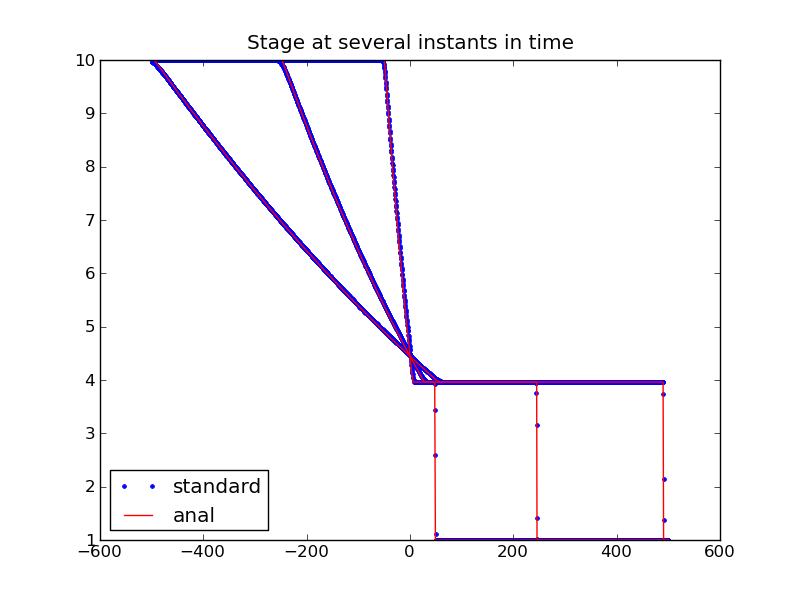
\includegraphics[width=0.9\textwidth]{stage_plot.png}
\end{center}
\caption{Stage results}
\end{figure}


\begin{figure}[h]
\begin{center}
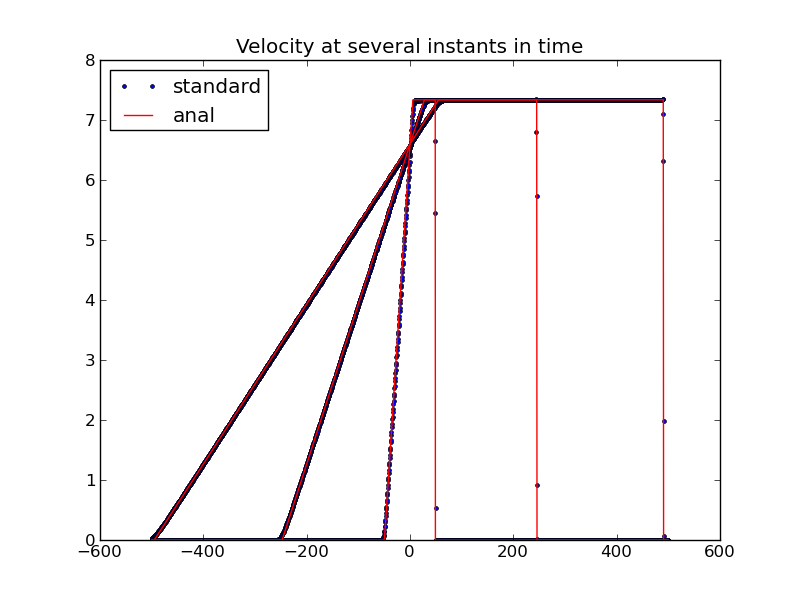
\includegraphics[width=0.9\textwidth]{xvel_plot.png}
\end{center}
\caption{Velocity results}
\end{figure}


\endinput
}
\newcommand{\cfl}{\UScore{1.0}}
\newcommand{\alg}{\UScore{tsunami}}
\newcommand{\majorR}{\UScore{1.3.0_beta}}
\newcommand{\minorR}{\UScore{8581}}
\newcommand{\timeR}{{Tue Sep 18 15:39:06 2012}}


%=========================================
\begin{document} 
%=========================================

\title{Automated Report on the Performance of \anuga{} on (all) Validation Test Problems}
\author{Sudi Mungkasi, Stephen Roberts, Gareth Davies, Rudy vanDrie}    %Type your name(s) here! 
\maketitle
\tableofcontents

%======================
\chapter{Introduction}
%======================
\anuga{} is a free and open source software developed by Roberts and collaborators from the Australian
National University (ANU) and Geoscience Australia (GA). It is devoted to fluid flow simulations,
especially shallow water flows, such as floods, tsunamis and dam breaks. The official website of
\anuga{} is \verb http://anuga.anu.edu.au .



The method implemented in \anuga{} is a numerical finite volume method used to
solve the shallow water equations. Some mathematical explanation of the method
is given in the \anuga{} User Manual~\cite{RNGS2010}. In two dimensions, the
domain is discretised into finite number of triangular elements. \anuga{}
then evolves the conserved quantities (water depth and momenta) with respect
to time to obtain the numerical solution to a given problem. The evolution
is based on the given quantity and flux values. The numerical flux used in
\anuga{} is the Kurganov's flux~\cite{KNP2001, KL2002}. The boundary conditions
that we use in this work include reflective, transmissive, Dirichlet
and time boundaries.


The results in this report were produced by \anuga{} version \majorR{} from svn
repository revision \minorR{} at time \timeR.
The flow algorithm used was \alg{}, unless otherwise stated explicitly. 

To get an automated report, 
we can run either run individual tests or the complete (whole) test.

To do an individual test, we can run the python module \\
\verb produce_results.py \\
available in the corresponding test directory. The module will do the 
numerical simulation of the given problem, plot the simulation 
results in png files, and typeset the corresponding 
individual automated report. The individual automated report is in 
the pdf file \verb report.pdf  saved in the same directory.

To do the complete test, we can just run the python module \\
\verb validations_produce_results.py \\
available in the directory \\
\verb validation_tests/reports \\
Similar to the module for an individual test, this python module 
will do the numerical simulations of all the given problems, 
plot results in png files and save them in its corresponding directory, 
and finally type-set the complete report. The complete automated report is saved in the
\verb validation_tests/reports   directory.

The simulation results can be analysed qualitatively and quantitatively. 
Qualitative analysis can be done by investigating the plots of 
the results whether they are physical or not, and whether the 
behaviour is the same as we expected. Quantitative analysis can 
be conducted by checking the numerical error. 

We have also provided a python script \verb run_auto_validation_tests.py in 
the \verb validation_tests  directory which will run a subset of the available tests 
having sensible ``correct'' results to test against.

The main parameters in the validations are the Courant--Friedrichs-Lewy (CFL) 
number and the flow algorithm. They are spelled 
\verb cfl  and \verb alg  respectively in the python module \\
\verb parameters \\
which is available in the \\
\verb anuga.validation_tests \\
module. In the default setting, we set the CFL to be $1.0$ and 
the flow algorithm to be \verb DE0  (second order in space and first order in time). 
The complete available flow algorithms are as follow:
\verb 1_0 ,
\verb 1_5 , 
\verb 1_75 , 
\verb 2_0 , 
\verb 2_0_limited , 
\verb 2_5 ,
\verb tsunami , 
\verb yusuke , 
\verb DE0 , 
\verb DE1 , 
\verb DE2 .

They can be found in \\
\verb \anuga_core\source\anuga\shallow_water\shallow_water_domain.py .



The report is organised as follows. We collect a number of tests against
analytical exact solutions in Chapter~\ref{ch:ana}. Tests against other
reference data or solutions are given in Chapter~\ref{ch:ref}.
We provide explanations on how to add new tests in the Appendix.

%======================
\chapter{Tests against analytical exact solutions} \label{ch:ana}
%======================

\inputresults{../analytical_exact/dam_break_dry}
\inputresults{../analytical_exact/dam_break_wet}
\inputresults{../analytical_exact/avalanche_dry}
\inputresults{../analytical_exact/avalanche_wet}
\inputresults{../analytical_exact/carrier_greenspan_periodic}
\inputresults{../analytical_exact/carrier_greenspan_transient}
\inputresults{../analytical_exact/deep_wave}
\inputresults{../analytical_exact/mac_donald_short_channel}
\inputresults{../analytical_exact/parabolic_basin}
\inputresults{../analytical_exact/paraboloid_basin}

\inputresults{../analytical_exact/runup_on_beach}
\inputresults{../analytical_exact/runup_on_sinusoid_beach}
\inputresults{../analytical_exact/landslide_tsunami}

\inputresults{../analytical_exact/lake_at_rest_immersed_bump}
\inputresults{../analytical_exact/lake_at_rest_steep_island}
\inputresults{../analytical_exact/river_at_rest_varying_topo_width}
\inputresults{../analytical_exact/rundown_mild_slope}
\inputresults{../analytical_exact/rundown_mild_slope_coarse}
\inputresults{../analytical_exact/subcritical_over_bump}
\inputresults{../analytical_exact/subcritical_flat}
\inputresults{../analytical_exact/transcritical_with_shock}
\inputresults{../analytical_exact/transcritical_without_shock}
\inputresults{../analytical_exact/supercritical_over_bump}
\inputresults{../analytical_exact/trapezoidal_channel}

%%======================
\chapter{Tests against reference data or solutions} \label{ch:ref}
%%======================
\inputresults{../experimental_data/dam_break_yeh_petroff}
\inputresults{../experimental_data/okushiri}

\inputresults{../behaviour_only/lid_driven_cavity}
\inputresults{../behaviour_only/weir_1}
\inputresults{../behaviour_only/bridge_hecras}
\inputresults{../behaviour_only/lateral_weir_hecras}
\inputresults{../behaviour_only/tides_hecras}

\inputresults{../other_references/radial_dam_break_dry}
\inputresults{../other_references/radial_dam_break_wet}


%======================
\appendix
%======================
%======================
\chapter{Adding New Tests}
%======================


To setup a new validation test, create a test directory under one of 
the validation directories. In that directory there should be the test code, a
\TeX{} file \texttt{results.tex} and a python script
\texttt{produce\_results.py}, which runs the simulation and produces the
outputs. Copy the format from one of the other test directories. 

In this \TeX{} file, \texttt{report.tex}, add a line
\begin{verbatim}
\inputresults{../Directory/Name}
\end{verbatim}



\section{Algorithm Parameters}
Note that parameters can be communicated from the \verb|local_parameters.py|
file in the \verb|validation_tests/reports| directory. If there is no file
\verb|local_parameters.py| then the parameters are taken from the
\verb|anuga.validation_utilities.parameters|. 

In particular the
values of \verb alg  (flow algorithm) and \verb cfl  (CFL Condition)
are passed as command options when calling \verb produce_results.py  in the
test directories.

Within \anuga{} script you can obtain command line parameters via
\begin{verbatim}
args = anuga.get_args()
alg = args.alg
verbose = args.verbose
\end{verbatim}
to obtain the values of \verb alg (flow algorithm) and \verb verbose (flag)

You can pass though the standard parameters as follows
\begin{verbatim}
from anuga.validation_utilities.parameters import alg
from anuga.validation_utilities.parameters import cfl
\end{verbatim}

\pagebreak
\section{Generic form of \texttt{produce\_results.py}}

The \texttt{produce\_results.py} files in the test directories should have the
following general form

\begin{verbatim}
import anuga
from anuga.validation_utilities import produce_report

args = anuga.get_args()

produce_report('run_simulation.py', args=args)
\end{verbatim}


%======================
% bibliography
%======================

\bibliographystyle{plain}
\bibliography{bibliography}

\end{document}
